\documentclass[12pt,a4paper]{report}
\usepackage[utf8]{inputenc}
\usepackage[inner=5cm,outer=2.5cm,bottom=3cm,top=2.5cm,pdftex]{geometry}
\usepackage{setspace}
\usepackage{graphicx}
\usepackage{rotating}
\usepackage[page]{appendix}
\usepackage{float}
\usepackage[font=small,labelfont=bf]{caption}
\usepackage{subfigure}
\usepackage{titlesec}
\usepackage[hidelinks]{hyperref}
\usepackage{listings}
\usepackage{textcomp}
\usepackage{fancyhdr}
\usepackage{multirow}
\usepackage{verbatim}	%makes it possible to comment out a section of text by using \begin{comment}...\end{comment}
\usepackage[table,xcdraw]{xcolor}
\usepackage{pifont}
\usepackage{mathptmx}
\usepackage{amsmath}
\usepackage{wrapfig}
\usepackage{ragged2e}
\usepackage[nottoc,notlot,notlof]{tocbibind}
\usepackage[english]{babel}
\usepackage[final]{pdfpages}

\definecolor{rockwoolcolor}{RGB}{0,0,0}

\makeatletter
\providecommand\add@text{}
\newcommand\tagaddtext[1]{%
  \gdef\add@text{#1\gdef\add@text{}}}% 
\renewcommand\tagform@[1]{%
  \maketag@@@{\llap{\add@text\quad}(\ignorespaces#1\unskip\@@italiccorr)}%
}
\makeatother

% Style chapter headings for preface and toc.
\setlength{\headheight}{15pt}
\titlespacing*{\chapter}{0pt}{0pt}{4ex}
\titleformat{\chapter}[display]
 {\bfseries\Large}
 {}
 {0pt}
 {\color{rockwoolcolor}\titlerule[2.0pt]\vspace{2ex}\filright\color{black}}
 [\color{rockwoolcolor}\vspace{2ex}{\titlerule[2.0pt]}]


\setstretch{1.25}
\begin{document}
\begin{titlepage}

\newcommand{\HRule}{\color{rockwoolcolor}\rule{\linewidth}{0.75mm}\color{black}} % Defines a new command for the horizontal lines, change thickness here

\center % Center everything on the page
 
%----------------------------------------------------------------------------------------
%	HEADING SECTIONS
%----------------------------------------------------------------------------------------
\ \\[1.5cm]
\textsc{\LARGE BI Norwegian Business School}\\[1.5cm] % Name of your university/college
\textsc{\Large GRA 41351 Decision Theory and System Dynamics}\\[2.5cm] % Major heading such as course name


%----------------------------------------------------------------------------------------
%	TITLE SECTION
%----------------------------------------------------------------------------------------

\HRule \\[0.4cm]
{ \huge \bfseries Waste Sorting Simulation Model for \\[0.5cm] Oslo Municipality}\\[0.4cm] % Title of your document
\HRule \\[2.5cm]
 
%----------------------------------------------------------------------------------------
%	DATE & PLACE SECTION
%----------------------------------------------------------------------------------------

{\large \textbf{Date of submission:}\\  \today}\\[1cm] % Date, change the \today to a set date if you want to be precise
{\large \textbf{University:}\\  BI Nydalen}\\[3cm] % Date, change the \today to a set date if you want to be precise
 
%----------------------------------------------------------------------------------------

\textit{This paper is a part of the MSc programme at BI Norwegian Business School. The school takes no
responsibility for the methods used, results found and conclusions drawn.}
\vfill % Fill the rest of the page with whitespace

\end{titlepage}
{\RaggedRight
\pagestyle{fancy}

% empty default settings for fancy layout
\fancyhf{}

% table mark commands
\newcommand{\cmark}{\textcolor{green!80!black}{\ding{51}}}
\newcommand{\xmark}{\textcolor{red}{\ding{55}}}
\newcommand{\plusmark}{\textcolor{green!80!black}{\textbf{+}}}
\newcommand{\minusmark}{\textcolor{red}{\textbf{-}}}

% chapter, section, header and footer layout
\renewcommand{\sectionmark}[1]{\markright{\thesection ~ \ #1}}
\renewcommand{\chaptermark}[1]{\markboth{ #1}{}}
\renewcommand{\headrulewidth}{0.5pt}
\renewcommand{\footrulewidth}{0.5pt}

%head setting
%\fancyhead[L]{\textcolor{black} {\rightmark}}
\fancyfoot[C]{\textcolor{black} {\thepage}}

% Redefine the plain page style - used when the page is a chapter
\fancypagestyle{plain}{%
  \fancyhf{}%
  \renewcommand{\headrulewidth}{0pt}% Line at the header invisible
  \renewcommand{\footrulewidth}{0.5pt}% Line at the footer visible
  \fancyfoot[C]{\textcolor{black} {\thepage}}
}

% Avoid hyphenating
\tolerance=10
\emergencystretch=\maxdimen
\hyphenpenalty=10000
\hbadness=10000

\pagenumbering{roman}
\chapter*{Abstract}
The main objective of this paper is analyzing waste sorting behavior and the different factors which influence waste sorting behavior in practice. The reasoning behind this is to help Oslo municipality with reaching a material recycling rate of 50\% by 2030. 

\indent \newline 
The target group consists of 20-39 year old's, not coming from Asia, Africa, Latin-America and Eastern Europe outside of EU. This represents approximately 27\% of all Oslo citizens, and is adjusted for in the simulation model. This means that the model will not be able to reach a realistic material recycling rate of 50\%.

\indent \newline 
A causal loop diagram is presented in order to give an overview of the different variables and their relationships. This includes both positive and negative links on waste sorting behavior. 

\indent \newline 
The simulation model was developed through expanding the existing stocks and flows model with findings from the causal loop diagram. Five initiatives are displayed in the model and consists of increasing advertising effectiveness, increasing the number of waste containers (new quality), implementing smart waste containers (improvements), utilizing economic incentives and increasing frequency of waste collection. The simulations show a "base case" scenario, with a resulting material recycling rate of 31.69\%, while the top three initiatives are increasing the number of waste containers, increasing frequency of waste collection and implementing smart waste containers, with a respectively recycling rate of 36.53\%, 34.4\% and 33.86\%.

\indent \newline 
A sensitivity analysis was performed in order to test the initiatives in different scenarios, which did not the change the recommended suggestions. 

\setcounter{tocdepth}{2}
\tableofcontents
%\addtocontents{toc}{~\hfill\textbf{Page}\par}
\listoftables

% ----------- CHAPTERS ----------------

% Parts
\cleardoublepage
% Style chapter headings.
\titleformat{\chapter}[display]
 {\bfseries\Large}
 {}
 {0pt}
 {\color{rockwoolcolor}\titlerule[2.0pt]\vspace{2ex}\filright\color{black} \thechapter . }
 [\color{rockwoolcolor}\vspace{2ex}{\titlerule[2.0pt]}]
\pagenumbering{arabic}
\setcounter{page}{1}

\renewcommand{\cleardoublepage}{}
\renewcommand{\clearpage}{}
\centering
\justify
\chapter{Introduction}
The following report examines three different boarding procedures with the objective of finding a more efficient boarding policy. The background for the research is based on the views many people have today regarding the process of boarding a plane. Many travelers find the process inefficient and annoying, where they are spending a lot of time in queues. This involves wasting time at the gate and in the corridor of the airplane, waiting for people to store their luggage. In order to reduce costs associated with flight delays, the first two simulation methods will be analysed in terms of identifying potential bottlenecks and other elements of the boarding procedures which can be carried out in a more efficient way. This will lead to a third and final simulation method where the potential improvements from the first two will be implemented.   

\indent \newline 
The next chapters of the report will start by explaining how relevant data have been collected, certain assumptions which have been made and the build-up of the simulation methods. Different scenarios are then proposed, consisting of certain conditions the first two boarding methods will be simulated under. Further, performance metrics are described and results of the first two simulations presented, before going into the third simulation method. Lastly, recommendations will be given on how airlines can implement a more efficient boarding policy.   



\chapter{Data Collection and Assumptions}
To be able to carry out the simulation methods in a realistic way, most parts of the models are based on data collected from sources online, conversations with the Assistant Duty Manager at Avinor, Marit Kristoffersen \cite{marit} and information given in the assignment. However, some parts are based on subjective assumptions which will be explained in further detail in the following section. 

\section{Data from the Assignment}
\subsection{Airplane Configuration}
Data regarding initial model parameters have been collected from information given in the assignment. This involves an airplane configuration consisting of 20 rows, 6 seats per row and 1 aisle. The plane occupancy is always 100\%, which means that 120 passengers are boarding the plane.

\subsection{Time Measures}
The time it takes for a passenger to walk from one row to the next is based on a triangular distribution measured in seconds, where {min; mode; max} = {1.8; 2.4; 3}. The time it takes for a passenger to sit without interference is also triangular distributed, measured in seconds, where {min; mode; max} = {6; 8; 10}. An important factor in the simulation is the time it takes a passenger to store luggage, and is based on the following formula:
\begin{figure}[H]
\centering
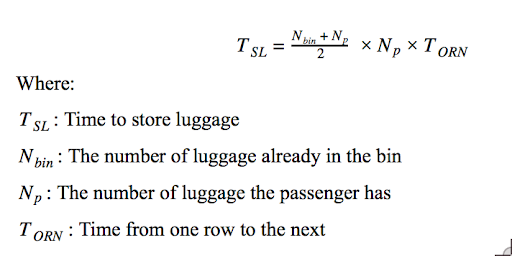
\includegraphics [scale=0.42,angle=360]{figures/unnamed.png}
\label{fig:unnamed}
\end{figure}
These criteria were incorporated into the models by changing the passengers’ speed according to the distance between the two consecutive rows, in case (1), and the distance between the center of the aisle and a middle seat, in case (2).

\section{Data from other Sources}
\subsection{Passengers Walking Speed}
People's average walking pace depends on the age of the person. Research has shown a speed ranging from approximately 1 meters/second to 1.5 meters/second \cite{speed}. Passengers in the model have therefore been set with a comfortable speed through a uniform distribution measured in meters per second, where {min; max} = {1.0; 1.5}. The speed applies only for situations where the passengers are able to walk uninterrupted. How fast passengers are moving in the aisle inside of the airplane is based on the time from one row to the next and the distance between two rows. The speed was calculated with a triangular distribution measured in meters per second, where {min; mode; max} = {0.94; 1.17; 1.56}. 

\subsection{Hand Luggage per Passenger}
There are different policies regarding the amount of hand luggage passengers are allowed to carry with them on an airplane. Searching the biggest airline's policies shows that it is common either to allow for 1 cabin bag + 1 personal item (laptop/handbag) or just 1 cabin bag \cite{luggage}. Based on this information, the simulation methods allow for passengers carrying up to 2 items of hand luggage.   

\subsection{Bin Capacity}
Based on personal experience, a common problem in the boarding process is the lack of space in the airplane bins, especially in situations where the airplane is fully occupied. One of the authors has a family member (Marit Kristoffersen) who has for many years worked in different roles at Oslo Airport, Gardermoen, and is currently working as an Assistant Duty Manager for Avinor. She was contacted in order to verify the assumption. She explained that this is a common issue among the airlines and an important factor to the boarding time. Hence, the simulation models consider a bin occupancy of 100%. 

\subsection{Data Sets}
In order to optimize the input of data used in the models and to make the scenarios easier to manage, data sets were created in excel and imported into the models. The data sets contain the values for various parameters used in the simulations. 

\chapter{Model Structure}
The following chapter describes the build-up of the first two models, with regards to the use of libraries, agents, blocks and important variables and parameters. The structure of both models is divided into three parts: the waiting area, service lines and the inside of the airplane. The models contain three different types of agents, namely passengers, bins and seat blocks. These have been created in order to control key parts of the simulations, and will be described in more detail in the next section. Furthermore, the pedestrian library was used to simulate the passenger flow in the different sequences of the boarding process. 

\section{Model 1 - Boarding in Blocks}
The first model simulates a commonly used boarding strategy among airlines today, where passengers are called to board in groups, and within each group get on board in a random sequence. The model contains an excel-file, where 120 passenger IDs are assigned to specific seats, classes, boarding sequence, luggage quantity, colors, which bins to use and if the seat is located by the window, middle or aisle. The seating is divided into three groups (classes), which are passengers with special needs (seated in row 1), first class (seated in row 2-5) and economy class (seated in row 6-20). There are also "gold" passengers who don't have to get in line. The boarding sequence is prioritized in the following order: 1. Special needs, 2. First class/gold passenger, 3. Economy class back (row 12 - 20), 4. Economy class front (6 - 11). To keep track of the different groups while carrying out the simulation, passengers within each group are associated with a specific color. Special needs are red, first class blue, gold passengers golden and economy class green. 

\subsection{Airplane Layout}
The inside of the airplane consists of 120 seat nodes representing passengers seat locations. These are divided into 40 seat blocks and separates seats located on the left and right side of the aisle. There are 14 storage bins, where one bin is associated with 3 rows and has  a capacity of storing 9 luggage items. This applies for the first 12 bins, where the last 2 bins are associated with 2 rows.

\subsection{Passenger Source Block}
The model starts with a passenger source block, where 120 passengers are created and arrive at the waiting area with an arrival rate of 1 per second. This block assigns each passenger created with the data in the excel file. 

\subsection{Waiting Area}
When the passengers arrive in the waiting area they wait between 1 and 3 minutes. While they are waiting, the passengers are added to a collection in order to keep track of passengers waiting to board. Next, in the ped select output block the passengers are checking if they can board. This is based on a function where passengers are prioritized as described in the previous section. As long as the passengers with special needs have boarded, the rest of the passengers can start boarding if there are less than 8 people with higher priority in the boarding queue. If there are more than 8 people in the queue, they will wait between 5 and 20 seconds before checking again.   

\subsection{Service Area}
The ped service block is visualized through a single queue where passengers have to show their documentation in order to board the plane. Passengers who exit the queue are removed from the collection containing passengers waiting to board, which enables passengers with lower priority to start boarding. Then they start moving towards the start of the aisle inside the plane.

\subsection{Storing Luggage}
When passengers arrive at the start of the seat rows, they first go to the bin location associated with their seat block. The luggage storing process is represented through the check bin block, where passengers who do not have any luggage can proceed to sit down in their seats. If the passenger has luggage and there is available space in the bin, the luggage will be stored and the passenger is then seated. In the case where the bin is full, the passenger will check the nearest bins. If there is available space, they will store their luggage there and go to their seats. 

\indent\newline
In order to make passengers stop and wait for others who are storing luggage, the passengers who are storing luggage checks who is in front of them and who is behind them, and is then added to two collections. This is done by calculating the distance between the passenger checking, and other surrounding passengers within a certain range. A negative distance means that the passengers are located behind, while a positive distance means that passengers within the range are in front of the passenger checking. If a passenger has someone in front of them storing luggage, they will slow down their walking speed, move up towards them, but not pass them. A limitation in the model is that it does not account for a situation where the total bin capacity is exceeded. On the other hand, this can sometimes be resolved by storing some of the luggage beneath the seats.   

\subsection{Letting Passengers get to their Seats}
An important part of the boarding process is to simulate passengers getting up from their seats to let another passenger in. A combination of a ped select output block and two ped wait blocks is used to do this. If there are passengers already seated in the row, and if they are interfering with the passenger trying to get to his or her seat, they will get up from their seats and move into the aisle.  

\subsection{Colors}
There are several variables (constants) regarding colors included in the model. The purpose is to help visualize different states in the model. When passengers are storing luggage, the color of the passengers turn pink, and when they are searching for another bin the color changes to purple. In situations where they have to get up from their seats to let another passenger in, they turn violet. Finally, when passengers are seated they change color to white.    

\section{Model 2 - Steffen's Method}
The second model is a boarding method proposed by Steffen J. who is a researcher on boarding problems. The method involves passengers being called to board the plane in a given sequence. The boarding sequence works as follows: The first passenger called to board is seated at the last row by the window on the right side of the aisle. Then the second passenger is also seated at the right side by the window, but two rows before the first passenger. The process continues for one side of the plane and is repeated on the other side, again starting with the window seats. In summary, the window seats are filled up first, then the middle and lastly the seats in the aisle:

\begin{table}[H]
  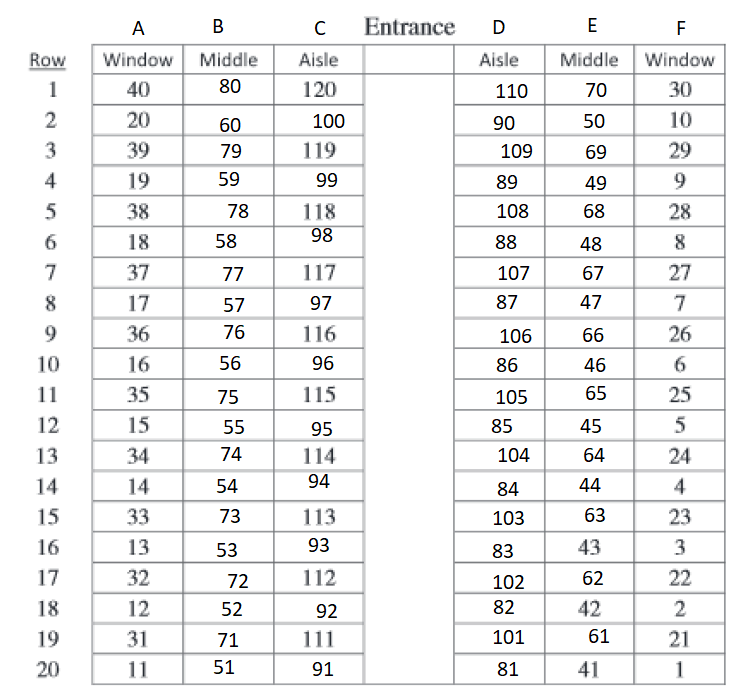
\includegraphics[width=0.75\textwidth]{tables/table1.png}
  \caption{Steffen's Method}
  \label{tbl:table1}
\end{table}

The structure of the model is based on the same logic as in the first model, which means that it consists of a waiting area, service area and the inside of the plane. However, there are some elements different from the first model, which will be explained next.

\subsection{Data from the Excel-File}
The passenger IDs in the excel-file are associated with a different seat location, and represent the specific boarding sequence as proposed by Steffen J. This means that passenger ID 1 is given seat number 20F, passenger ID 2 is given seat number 18 F etc. The model does not take into consideration the different groups of passengers (classes) and is visualized through all of the passengers having the same color.

\subsection{Service Area}
The queue to the boarding service is constructed as a serpentine queue, opposed to the service queue in the first model. The reasoning behind this is to avoid a situation where there are passengers entering the plane before everyone is present in the waiting area. Another reason is to create a longer queue, so the airport employees can make sure that the passengers are boarding in the correct order. Since the two models differ in this part, it will be taken into consideration when comparing the time measurement between the models. 



\chapter{Performance Metrics}
The two models described in chapter 3 have very distinct features, from the grouping of the passengers according to their priority level to the order of seats being occupied as passengers come inside the airplane. In order to check which of the two has a more efficient boarding system, several statistics were computed at the end of each model's run time.

\indent\newline
First off, the total boarding time. This was considered as the time between the first passenger starting to board the plane and the last passenger sitting down, and it was measured with the help of TimeMeasurementStart component, a variable called "timeBoardStarted" that stores the time the first passenger showed their documentation and a function that keeps computing the difference between the present and that stored time, until all passengers are seated.
However, it is also important to understand why exactly a certain model’s boarding system finishes quicker. So additionally, four other performance metrics were focused on analyzing four different sections of the models: a) the pre-boarding time; b) the time prior to a passenger showing their documentation; c) the time related to passengers storing their luggage; d) the time it takes for passengers to sit down in their respective seats. 

\indent\newline
The time differences per passenger were obtained through placing TimeMeasurement components before or after specific blocks and were graphically displayed in Histograms and also Line Plots, which required storing them in data sets. Pie charts were also included in the Statistics window, with a different purpose in mind: by comparing the total number of times any passenger sits down or gets up from their seat, it is possible to know how inconvenient seat interference really is. Bins being full is another great inconvenience for passengers with luggage, which the second pie chart highlights, by counting the number of passengers that store their bags in a bin other than the one above their seat. Both pie charts’ inputs came from variables whose value got incremented every time a passenger entered blocks such as "pedGoToOtherBin" or "pedWaitOnSeat", for example.


\chapter{Results}
Using the original data set (“PassengersNormal”) as the basis of comparison, several conclusions could be drawn regarding the models' efficiency or inefficiency and the reasons for it. The time differences for each specific measurement mentioned in chapter 4 were summarized in the following table:
\begin{table}[H]
  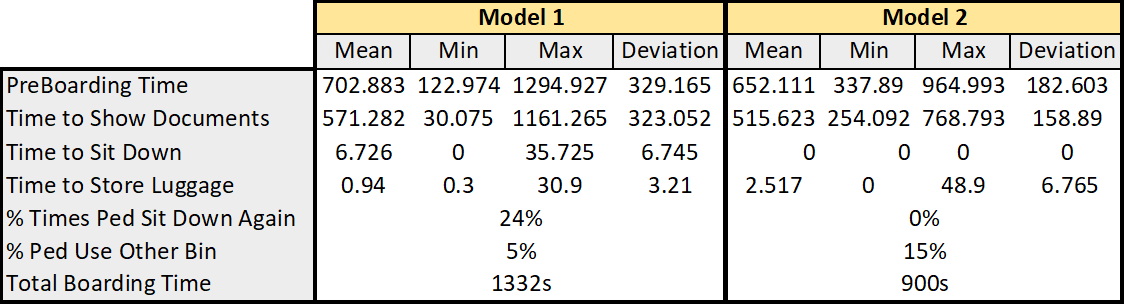
\includegraphics[width=1.0\textwidth]{tables/statistics.png}
  \caption{Time Statistics - Model 1 \& 2}
  \label{tbl:statistics}
\end{table}
Starting with the pre-boarding time, in the first model most passengers have to wait for groups with higher priority to enter the plane first, and even though the second model's system establishes an even more specific entrance sequence, the average time passengers spend waiting to show their documentations from the moment they get to the waiting area is 702.883 seconds for Model 1 and 652.111 seconds for Model 2. The same happens when just considering how long it takes for passengers to get to the staff verifying the documentation. This can probably be explained by both models checking if everyone has arrived at the waiting area before enabling passengers to form a queue. It should be noticed, however, that the lowest waiting time values were obtained in Model 1 as, because of the data set file, the first passengers to arrive are people with special needs, who can immediately start boarding.

\indent\newline
Moving onto the time passengers take to sit down, as expected, there is absolutely no interference in Model 2 in the sense that no passenger has to get up from their seat in order to let another passenger sit down in the same sitting block. On the other hand, Model 1 does not avoid nor minimize this concern. At the most extreme case, a passenger already standing in front of their sitting block still had to wait 35.725 seconds to sit down. Consequently, whereas in Model 1 24\% of the passengers kept leaving their seat and sitting down again, in Model 2 this percentage is reduced to 0.
Interestingly enough, Model 1 did overcome Model 2 in one aspect: the time spent storing luggage. Neither model was prepared to optimize the search for other bins when the one above the passenger's seat is full and so in both models passengers move along the aisle trying to store their bags. But neither one is clearly superior either. To put it simply, the particular data set associating the amount of luggage per passenger turned out more favorable for Model 1 than for Model 2, resulting in an average searching time of 0.94 seconds for the first and of 2.51 seconds for the latter. This was also reflected in the percentage of passengers looking for alternative bins: 15\% for Model 2 and only 5\% for Model 1. So not only did passengers take more time to store their luggage but also more passengers had trouble finding room left for their belongings.
\indent\newline
This said, overall Model 2 was much more efficient, resulting in a total boarding time of 900 seconds whereas Model 1 took longer to finish: 1332 seconds.


\chapter{Model 3}
Each model has its own advantages and disadvantages. Boarding by blocks allows passengers to sit according to their own preference, be it staying with their families or friends or sitting in a specific area of the airplane. This freedom makes it impossible to optimize problematic aspects such as the ones previously discussed. On the other hand, Steffen’s method is much more strict in regards to where each passenger is seated, ignoring their preference or special condition in order to reduce interference within the same three seat block. The subsequent higher efficiency was obvious in chapter 5, as the model did prove to be much more practical in sitting passengers down. However, it was also observed that in Model 1 passengers spent less time storing their luggage, which is definitely a problem that Steffen’s method ends up ignoring.

\indent\newline
This said, a third model was developed to optimize the luggage disposition inside the airplane while aiming for the unobstructed boarding sequence Model 2 excels at. The logic behind its boarding sequence can be divided into three steps:

\section{The Third Method Algorithm}
\subsection{Step 1: Assigning the passengers to a specific seat according to their luggage quantity}
This is a pre-boarding step. All passengers are distributed by the seats according to the quantity of luggage they have, in order to have the passengers with less luggage seated closer to the windows, and the passengers with more luggage seated closer to the aisle. This is because the less luggage they have, the less time they spend storing it and consequently the smaller the chances another passenger will arrive in the meantime and wait in the aisle. Once seated in their seats, passengers seated near the window won't need anything else. 

\indent\newline
The order of the quantity of luggage entering the airplane will then be: 0, 0, 0, 0, 0, 0, 0, 0, 0, 0, 0, 0, 0, 0, 0, 0, 0, 0, 0, 1, 1, 1, 1, 1, 1, 1, 1, 1, 1, 1, 1, 1, 1, 1, 1, 1, 1, 1, 1, 1, 1, 1, 1, 1, 1, 1, 1, 1, 1, 1, 1, 1, 1, 1, 1, 1, 1, 1, 1, 1, 1, 1, 1, 1, 1, 1, 1, 1, 1, 1, 1, 1, 1, 1, 1, 1, 1, 1, 1, 1, 1, 1, 1, 1, 1, 1, 1, 1, 1, 1, 1, 1, 1, 1, 1, 1, 1, 1, 1, 2, 2, 2, 2, 2, 2, 2, 2, 2, 2, 2, 2, 2, 2, 2, 2, 2, 2, 2, 2, 2. The following table shows the quantity of luggage associated to each one of the 120 seats:
\begin{table}[H]
  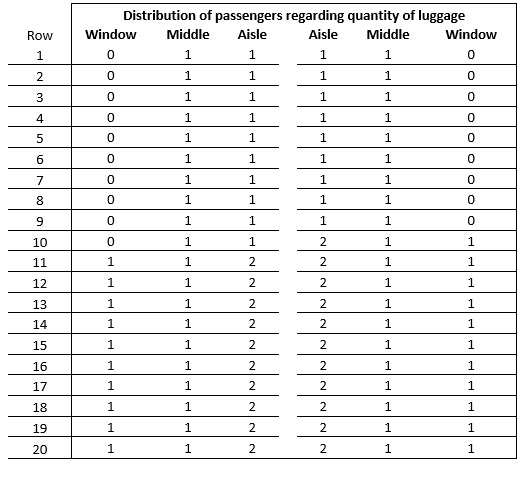
\includegraphics[width=0.75\textwidth]{tables/luggage.jpg}
  \caption{Luggage Distribution}
  \label{tbl:luggage}
\end{table}
\subsection{Step 2: Optimization}
This is also a pre-boarding step that tries to optimize the sequence defined in step 1, avoiding the need for passengers to change the bin as much as possible. The algorithm loops through the bins to simulate the luggage distribution inside the airplane and does the following:
\indent \newline
\begin{itemize}
\item If the bin's capacity is exceeded by 2 or more luggages, check if it's possible to change a passenger with 2 luggages that would be seated under this bin by a passenger with 0 luggage seated under a different bin with at least 2 available places.
\item If the bin's capacity is exceeded by just 1 luggage, check if it's possible to change  a passenger with 1 luggage that would be seated under this bin by a passenger with 0 luggage seated under a different bin with at least 1 available place
\item Update the boarding sequence of passengers 
\item Stop if no more passengers can be swapped.
\end{itemize}

\indent \newline
Some important observations about this step: since the algorithm's priority is to avoid the passengers need to change their respective bins, it is possible to change a passenger with luggage in an aisle seat with a passenger without luggage in a window seat. Also, a passenger will only change bin if it is possible to store all of his luggage in the candidate bin. 

\subsection{Step 3 Ordering the passengers according to Steffen’s Method}
After the arrangements in steps 1 and 2, the passengers will board according to the proposed method of Steffen.

\section{Improvements}
In order to check whether this new model is indeed an improvement from the previous two, the same performance metrics were used and the same passenger data set ("PassengersNormal") was chosen. By looking at the table below, it can be noticed that even though Model 3 did not differ much from Model 2 regarding the pre-boarding time and the waiting time to show documentation at the end of the queue, it succeeded in minimizing the time passengers spend storing their luggage, consequently reducing the total boarding time. This is also indicated by the percentage of passengers that end up using a bin other than the one above their seat, which was reduced from 15\% to 0\%, meaning that every passenger was able to store their belongings in their respective bin.


\begin{table}[H]
  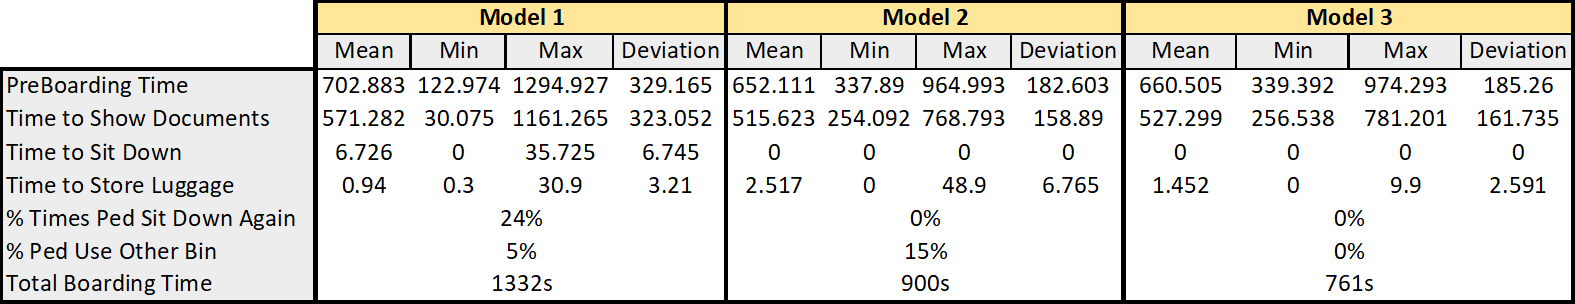
\includegraphics[width=1.0\textwidth]{tables/statistics2.png}
  \caption{Time Statistics - Model 3}
  \label{tbl:statistics2}
\end{table}


\chapter{Scenarios}
Finally, some experiments were conducted in order to compare the three models in different scenarios, all of which are related to luggage distribution as this seemed to be the most interesting efficiency factor.

\section{Different Luggage Distribution}
Apart from the original scenario, in which 19 passengers had 0 luggage, 80 passengers had just 1 luggage, and 21 passengers had 2 luggages, the data set "1LuggagePerPassenger\_2Only2" was tried out for the three models: 0 passengers had 0 luggage, 118 passengers had just 1 luggage and 2 passengers had 2 luggages. The results were arranged into the following table:

\begin{table}[H]
  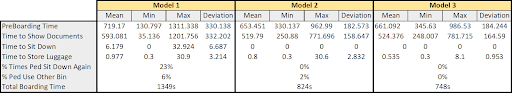
\includegraphics[width=1.0\textwidth]{tables/statistics3.png}
  \caption{Time Statistics - Scenario 1}
  \label{tbl:statistics3}
\end{table}

As suspected in Section 6, where Models 1 and 2 were compared based on the original dataset, the one performance metric for which Model 1 had a better result had indeed been due to chance, and not a specific more efficient feature of Model 1. Now that the amount of luggage each passenger carries has changed, the situation has turned out to be one where passengers spend, on average, 0.8 seconds storing their luggage in Model 2 and 0.977 seconds in Model 1, and where only 2\% of the passengers have to search for a different bin in Model 2, instead of 6\% in Model 1. Unsurprisingly, Model 3 maintains the highest efficiency result in most performance metrics.

\section{Concentration of luggage in a specific area of the plane}
Additionally, two other situations were tested, this time only for Model 1 and Model 2. In the first one (data set "ConcentrateLuggageBack"), the majority of luggage was carried by passengers seated at the back of the airplane, while in the second scenario (data set "ConcentrateLuggageFront"), the luggage was mostly assigned to bins at the front of the airplane. By comparing the performance metrics presented in the tables below with the results obtained in the original scenario, it can be immediately noticed that almost everything remained the same except for the luggage time. For both cases, passengers take much more time to store their belongings as the luggage is unevenly distributed among the bins. This is true for both models.

\begin{table}[H]
  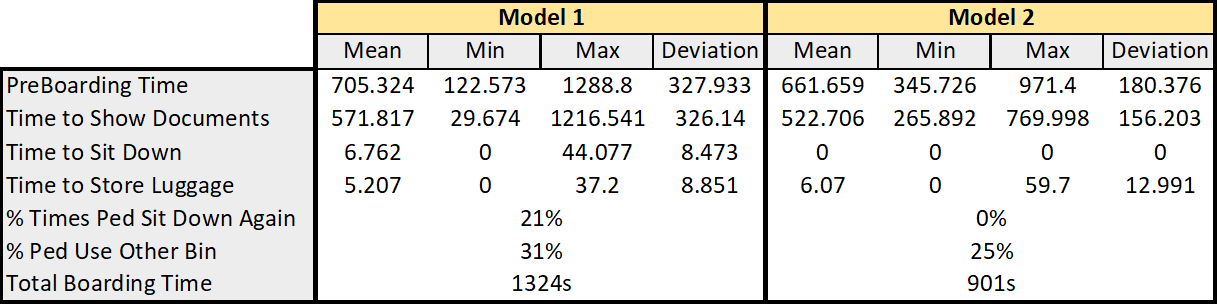
\includegraphics[width=1.0\textwidth]{tables/statistics4.png}
  \caption{Time Statistics - Scenario 2}
  \label{tbl:statistics4}
\end{table}

\begin{table}[H]
  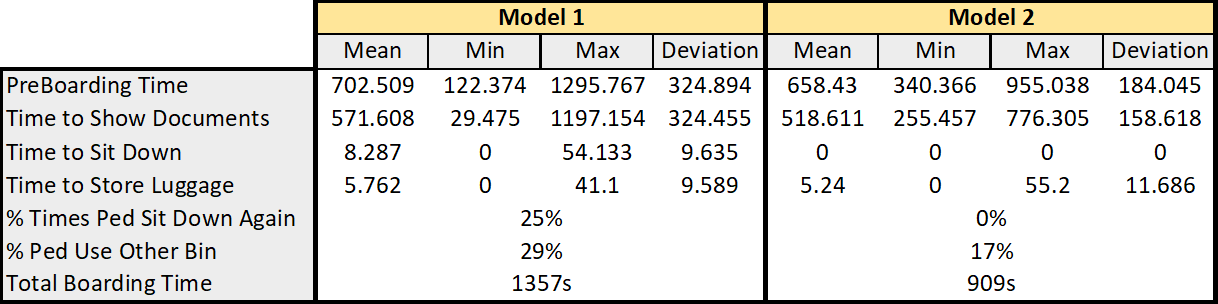
\includegraphics[width=1.0\textwidth]{tables/statistics5.png}
  \caption{Time Statistics - Scenario 3}
  \label{tbl:statistics5}
\end{table}	




\chapter{Conclusion}
This report examined two different boarding methods: one where passengers board in blocks and another where they enter the plane in a specific sequence (Steffen J's method). Upon analyzing their strengths and weaknesses, a third model was mostly based on Steffen's method to minimize its biggest inefficiency: the time spent looking for other bins with available space to store the passenger's luggage. This model succeeded to surpass the other two in almost every performance metric used.
Finally, with the help of different scenarios it could be concluded that none of the first two models has a specific feature that dictates a better performance regarding this luggage issue. Also, when the luggage is unevenly distributed along the airplane, this tends to result in a significantly worse performance that, surprisingly, does not worsen other problematic situations such as passengers having to leave their seats in order to let others pass.
Given the strong correlation between the total boarding time and issues related to the storage of luggage and seat interference, it is thus suggested that the performances in these two aspects are key measurements for boarding models.




\newpage
% chapter heading as preface and toc
\titleformat{\chapter}[display]
 {\bfseries\Large}
 {}
 {0pt}
 {\color{rockwoolcolor}\titlerule[2.0pt]\vspace{2ex}\filright\color{black}}
 [\color{rockwoolcolor}\vspace{2ex}{\titlerule[2.0pt]}]
 
\renewcommand\bibname{References}
\bibliographystyle{apalike}	% (uses file "plain.bst")
\bibliography{myrefs}		% expects file "mineReferanser.bib"
}

\end{document}
